\ifx\wholebook\relax\else

% --------------------------------------------
% Lulu:

    \documentclass[a4paper,12pt,twoside]{../includes/ThesisStyle}

	\usepackage[T1]{fontenc} %%%key to get copy and paste for the code!
%\usepackage[utf8]{inputenc} %%% to support copy and paste with accents for frnehc stuff
\usepackage{times}
\usepackage{ifthen}
\usepackage{xspace}
\usepackage{alltt}
\usepackage{latexsym}
\usepackage{url}            
\usepackage{amssymb}
\usepackage{amsfonts}
\usepackage{amsmath}
\usepackage{stmaryrd}
\usepackage{enumerate}
\usepackage{cite}
%\usepackage[pdftex,colorlinks=true,pdfstartview=FitV,linkcolor=blue,citecolor=blue,urlcolor=blue]{hyperref}
\usepackage{xspace}
%\usepackage{graphicx}
\usepackage{subfigure}
\usepackage[scaled=0.85]{helvet}
        
        
\newcommand{\sepe}{\mbox{>>}}
\newcommand{\pack}[1]{\emph{#1}}
\newcommand{\ozo}{\textsc{oZone}\xspace}
\newcommand\currentissues{\par\smallskip\textbf{Current Issues -- }}

\newboolean{showcomments}
\setboolean{showcomments}{true}
\ifthenelse{\boolean{showcomments}}
  {\newcommand{\bnote}[2]{
	\fbox{\bfseries\sffamily\scriptsize#1}
    {\sf\small$\blacktriangleright$\textit{#2}$\blacktriangleleft$}
    % \marginpar{\fbox{\bfseries\sffamily#1}}
   }
   \newcommand{\cvsversion}{\emph{\scriptsize$-$Id: macros.tex,v 1.1.1.1 2007/02/28 13:43:36 bergel Exp $-$}}
  }
  {\newcommand{\bnote}[2]{}
   \newcommand{\cvsversion}{}
  } 


\newcommand{\here}{\bnote{***}{CONTINUE HERE}}
\newcommand{\nb}[1]{\bnote{NB}{#1}}
\newcommand{\fix}[1]{\bnote{FIX}{#1}}
%%%% add your own macros 

\newcommand{\sd}[1]{\bnote{Stef}{#1}}
\newcommand{\ja}[1]{\bnote{Jannik}{#1}}
\newcommand{\na}[1]{\bnote{Nico}{#1}}
%%% 


\newcommand{\figref}[1]{Figure~\ref{fig:#1}}
\newcommand{\figlabel}[1]{\label{fig:#1}}
\newcommand{\tabref}[1]{Table~\ref{tab:#1}}
\newcommand{\layout}[1]{#1}
\newcommand{\commented}[1]{}
\newcommand{\secref}[1]{Section \ref{sec:#1}}
\newcommand{\seclabel}[1]{\label{sec:#1}}

%\newcommand{\ct}[1]{\textsf{#1}}
\newcommand{\stCode}[1]{\textsf{#1}}
\newcommand{\stMethod}[1]{\textsf{#1}}
\newcommand{\sep}{\texttt{>>}\xspace}
\newcommand{\stAssoc}{\texttt{->}\xspace}

\newcommand{\stBar}{$\mid$}
\newcommand{\stSelector}{$\gg$}
\newcommand{\ret}{\^{}}
\newcommand{\msup}{$>$}
%\newcommand{\ret}{$\uparrow$\xspace}

\newcommand{\myparagraph}[1]{\noindent\textbf{#1.}}
\newcommand{\eg}{\emph{e.g.,}\xspace}
\newcommand{\ie}{\emph{i.e.,}\xspace}
\newcommand{\ct}[1]{{\textsf{#1}}\xspace}


\newenvironment{code}
    {\begin{alltt}\sffamily}
    {\end{alltt}\normalsize}

\newcommand{\defaultScale}{0.55}
\newcommand{\pic}[3]{
   \begin{figure}[h]
   \begin{center}
   \includegraphics[scale=\defaultScale]{#1}
   \caption{#2}
   \label{#3}
   \end{center}
   \end{figure}
}

\newcommand{\twocolumnpic}[3]{
   \begin{figure*}[!ht]
   \begin{center}
   \includegraphics[scale=\defaultScale]{#1}
   \caption{#2}
   \label{#3}
   \end{center}
   \end{figure*}}

\newcommand{\infe}{$<$}
\newcommand{\supe}{$\rightarrow$\xspace}
\newcommand{\di}{$\gg$\xspace}
\newcommand{\adhoc}{\textit{ad-hoc}\xspace}

\usepackage{url}            
\makeatletter
\def\url@leostyle{%
  \@ifundefined{selectfont}{\def\UrlFont{\sf}}{\def\UrlFont{\small\sffamily}}}
\makeatother
% Now actually use the newly defined style.
\urlstyle{leo}



	\usepackage{amsmath,amssymb}             % AMS Math
% \usepackage[french]{babel}
\usepackage[latin1]{inputenc}
\usepackage[T1]{fontenc}
\usepackage[left=1.5in,right=1.3in,top=1.1in,bottom=1.1in,includefoot,includehead,headheight=13.6pt]{geometry}
\renewcommand{\baselinestretch}{1.05}

\usepackage{multicol}

% Table of contents for each chapter

\usepackage[nottoc, notlof, notlot]{tocbibind}
\usepackage{minitoc}
\setcounter{minitocdepth}{1}
\mtcindent=15pt
% Use \minitoc where to put a table of contents

\usepackage{enumitem}

\usepackage{aecompl}

% Glossary / list of abbreviations

%\usepackage[intoc]{nomencl}
%\renewcommand{\nomname}{List of Abbreviations}
%
%\makenomenclature

% My pdf code

\usepackage[pdftex]{graphicx}
\usepackage[a4paper,pagebackref,hyperindex=true]{hyperref}

\usepackage{pgfplotstable,booktabs,colortbl}
\pgfplotsset{compat=1.8}

% Links in pdf
\usepackage{color}
\definecolor{linkcol}{rgb}{0,0,0.4} 
\definecolor{citecol}{rgb}{0.5,0,0} 

% Change this to change the informations included in the pdf file

% See hyperref documentation for information on those parameters

\hypersetup
{
bookmarksopen=true,
pdftitle="Sista: a Metacircular Architecture for Runtime Optimisation Persistence",
pdfauthor="Clement BERA", 
pdfsubject="Thesis", %subject of the document
%pdftoolbar=false, % toolbar hidden
pdfmenubar=true, %menubar shown
pdfhighlight=/O, %effect of clicking on a link
colorlinks=true, %couleurs sur les liens hypertextes
pdfpagemode=None, %aucun mode de page
pdfpagelayout=SinglePage, %ouverture en simple page
pdffitwindow=true, %pages ouvertes entierement dans toute la fenetre
linkcolor=linkcol, %couleur des liens hypertextes internes
citecolor=citecol, %couleur des liens pour les citations
urlcolor=linkcol %couleur des liens pour les url
}

% definitions.
% -------------------

\setcounter{secnumdepth}{3}
\setcounter{tocdepth}{1}

% Some useful commands and shortcut for maths:  partial derivative and stuff

\newcommand{\pd}[2]{\frac{\partial #1}{\partial #2}}
\def\abs{\operatorname{abs}}
\def\argmax{\operatornamewithlimits{arg\,max}}
\def\argmin{\operatornamewithlimits{arg\,min}}
\def\diag{\operatorname{Diag}}
\newcommand{\eqRef}[1]{(\ref{#1})}

\usepackage{rotating}                    % Sideways of figures & tables
%\usepackage{bibunits}
%\usepackage[sectionbib]{chapterbib}          % Cross-reference package (Natural BiB)
%\usepackage{natbib}                  % Put References at the end of each chapter
                                         % Do not put 'sectionbib' option here.
                                         % Sectionbib option in 'natbib' will do.
\usepackage{fancyhdr}                    % Fancy Header and Footer

% \usepackage{txfonts}                     % Public Times New Roman text & math font
  
%%% Fancy Header %%%%%%%%%%%%%%%%%%%%%%%%%%%%%%%%%%%%%%%%%%%%%%%%%%%%%%%%%%%%%%%%%%
% Fancy Header Style Options

\pagestyle{fancy}                       % Sets fancy header and footer
\fancyfoot{}                            % Delete current footer settings

%\renewcommand{\chaptermark}[1]{         % Lower Case Chapter marker style
%  \markboth{\chaptername\ \thechapter.\ #1}}{}} %

%\renewcommand{\sectionmark}[1]{         % Lower case Section marker style
%  \markright{\thesection.\ #1}}         %

\fancyhead[LE,RO]{\bfseries\thepage}    % Page number (boldface) in left on even
% pages and right on odd pages
\fancyhead[RE]{\bfseries\nouppercase{\leftmark}}      % Chapter in the right on even pages
\fancyhead[LO]{\bfseries\nouppercase{\rightmark}}     % Section in the left on odd pages

\let\headruleORIG\headrule
\renewcommand{\headrule}{\color{black} \headruleORIG}
\renewcommand{\headrulewidth}{1.0pt}
\usepackage{colortbl}
\arrayrulecolor{black}

\fancypagestyle{plain}{
  \fancyhead{}
  \fancyfoot{}
  \renewcommand{\headrulewidth}{0pt}
}

\usepackage{algorithm}
\usepackage[noend]{algorithmic}

%%% Clear Header %%%%%%%%%%%%%%%%%%%%%%%%%%%%%%%%%%%%%%%%%%%%%%%%%%%%%%%%%%%%%%%%%%
% Clear Header Style on the Last Empty Odd pages
\makeatletter

\def\cleardoublepage{\clearpage\if@twoside \ifodd\c@page\else%
  \hbox{}%
  \thispagestyle{empty}%              % Empty header styles
  \newpage%
  \if@twocolumn\hbox{}\newpage\fi\fi\fi}

\makeatother
 
%%%%%%%%%%%%%%%%%%%%%%%%%%%%%%%%%%%%%%%%%%%%%%%%%%%%%%%%%%%%%%%%%%%%%%%%%%%%%%% 
% Prints your review date and 'Draft Version' (From Josullvn, CS, CMU)
\newcommand{\reviewtimetoday}[2]{\special{!userdict begin
    /bop-hook{gsave 20 710 translate 45 rotate 0.8 setgray
      /Times-Roman findfont 12 scalefont setfont 0 0   moveto (#1) show
      0 -12 moveto (#2) show grestore}def end}}
% You can turn on or off this option.
% \reviewtimetoday{\today}{Draft Version}
%%%%%%%%%%%%%%%%%%%%%%%%%%%%%%%%%%%%%%%%%%%%%%%%%%%%%%%%%%%%%%%%%%%%%%%%%%%%%%% 

\newenvironment{maxime}[1]
{
\vspace*{0cm}
\hfill
\begin{minipage}{0.5\textwidth}%
%\rule[0.5ex]{\textwidth}{0.1mm}\\%
\hrulefill $\:$ {\bf #1}\\
%\vspace*{-0.25cm}
\it 
}%
{%

\hrulefill
\vspace*{0.5cm}%
\end{minipage}
}

\let\minitocORIG\minitoc
\renewcommand{\minitoc}{\minitocORIG \vspace{1.5em}}

\usepackage{multirow}
\usepackage{slashbox}

\newenvironment{bulletList}%
{ \begin{list}%
	{$\bullet$}%
	{\setlength{\labelwidth}{25pt}%
	 \setlength{\leftmargin}{30pt}%
	 \setlength{\itemsep}{\parsep}}}%
{ \end{list} }

\newtheorem{definition}{D�finition}
\renewcommand{\epsilon}{\varepsilon}

% centered page environment

\newenvironment{vcenterpage}
{\newpage\vspace*{\fill}\thispagestyle{empty}\renewcommand{\headrulewidth}{0pt}}
{\vspace*{\fill}}



	\graphicspath{{.}{../figures/}}
	\begin{document}
\fi

\chapter{Sista Architecture}
\label{chap:architecture}
\minitoc

%Generic intro
The overall thesis focuses on the design and implementation of an optimising JIT compiler for Pharo, written in Pharo itself, running in the same runtime than the optimised application on top of the existing runtime environment. In this chapter, we detail the architecture designed and implemented to make it work.

%opt intro
Cogit was extended to detect hot spot through profiling counters in non optimised n-functions. When a hot spot is detected, Cogit immediately calls Scorch in Pharo. Scorch then looks for the best v-function to optimise based on the current stack, optimises it and installs the optimised version. To perform optimisation, Scorch may ask Cogit to introspect specific n-functions to extract type information and basic block usage from previous runs. Once installed, the VM can execute the optimised v-function at the next call to the function. As the VM runtime is hybrid between an interpreter and Cogit, the optimised v-function may be interpreted or compiled to an optimised n-function by Cogit. As optimised v-functions have accessed to operations not normally possible by v-functions, both the interpreter and Cogit were extended to support the new operations.

%deopt intro
Due to speculative optimisations, optimised v-functions may contain guards to ensure optimisation-time speculations are valid at runtime. If a guard fails, the execution stack needs to be deoptimised to resume execution with non optimised code. When an optimised n-frame needs to be deoptimised, Cogit maps the optimised n-frame to a single optimised v-frame, provides it to Scorch, which maps the optimised v-frame to multiple non optimised v-frames. Scorch may then discard the optimised v-function if guards are failing too often in it. Lastly, the execution can resume using non optimised v-functions.

%???
%MAYBE FIGURE WITH SCORCH COGIT BOTH SIDE IMAGE / VM

%%%%%%%%%%%%%%%%%%%%%%%%%%%%%%%%%%%%%%%%%%%%%%%%%%%%%%%%%%%%%%%%%%%%%%%%%%%%%%%%%%%%%%%%%%%%%%%%%%%%%%%%%%%%%%%%%%%%%%%%

\section {Function's optimisation}

%Intro
Cogit was extended to detect hot spots based on profiling counters. When a hot spot is detected, Cogit triggers a call-back to request Scorch to optimise a v-function based on the current stack. The overall design is then the following: Scorch interrupts temporarily the application green thread, finds a v-function to optimise based on the current stack, optimises it, installs the optimised version, and resumes the application. The optimised v-function installed will be executed at the next call of the function.

\subsection{Optimiser critical and background modes}

%TimeBeforePostPoning: problem so it's required
The optimiser may however require a significant amount of time to optimise a function. Indeed, optimising a function can take a long time in slow machines or when a pathological function is optimised. This can lead to an interruption of the main application for an amount time long enough to be noticed by the application's user. To experiment with the optimiser, we worked mainly using the development environment of Pharo (which is written in Pharo). In the case of a user-interface application like the Pharo IDE, it is \emph{very} annoying to see the application interrupted during half a second or more when multiple functions long to optimise are optimised in a row, it feels like the user interface is slow, lagging and unresponsive even though the overall code takes less time to execute.

%First solution: timeBeforePostponing, with constraint for long methods
To avoid the problem, we limited the time window of the optimiser to a small amount of time, configurable from the language. For the development tools, we limited it to 40 ms. The limitation is enforced by a high-priority green thread, set to stop the optimiser after the given amount of time. As the current tools are refreshing at 50Hz, it means that the optimiser, at worst, force the system not to refresh the screen twice. In practice, most v-functions are optimised in less than 40ms. However, we now have a significant problem: v-functions too long to optimise are not optimised at all.
%Didn't use frame before not to confuse graphic frames with stack frames.

%idle and postpone
Upon profiling, we noticed, as one would expect, that this user interface application spends a significant amount of time in idle\footnote{An application in idle means it has nothing to do, it is typically waiting for an event to do anything.}. We show for example in figure \ref{fig:ApplicationIdle} that the application is successfully executing code, then idle, then executing code again, etc. 

\begin{figure}[h!]
    \begin{center}
        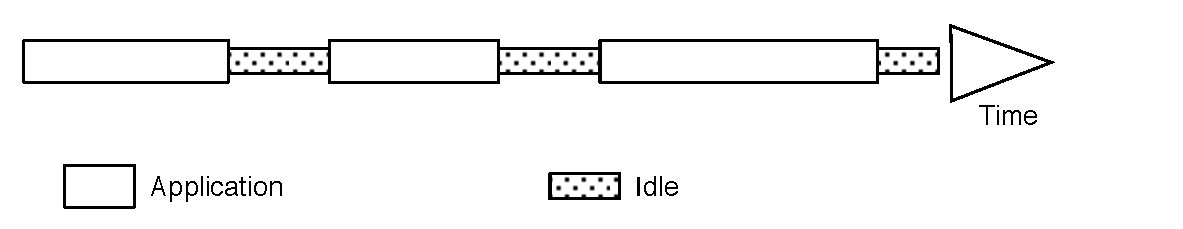
\includegraphics[width=0.9\linewidth]{ApplicationIdle}
        \caption{User interface application idle times}
        \label{fig:ApplicationIdle}
    \end{center}
\end{figure}

%background thread
Based on this result, we introduced a background green thread responsible for optimising the functions too long to optimise in the small time window. Hence, when the application would normally become idle, it starts by optimising such functions and becomes idle when no functions to optimise are remaining.

%Critical vs background
The optimiser can therefore be run in two mode. When a hot spot is detected, the optimiser is started in \emph{critical mode}. It has a limited amount of time to optimise a function based on the current stack. If the optimisation takes too long, the function to optimise is postpone to the background compilation queue. When the application becomes idle, if the background compilation queue is not empty, the optimiser is started in \emph{background mode}. In background mode, the optimiser is run in a low-priority green thread and is interrupted by any application green thread. When the optimiser has optimised all the functions in the compilation queue, it stops and the application becomes idle.

\begin{figure}[h!]
    \begin{center}
        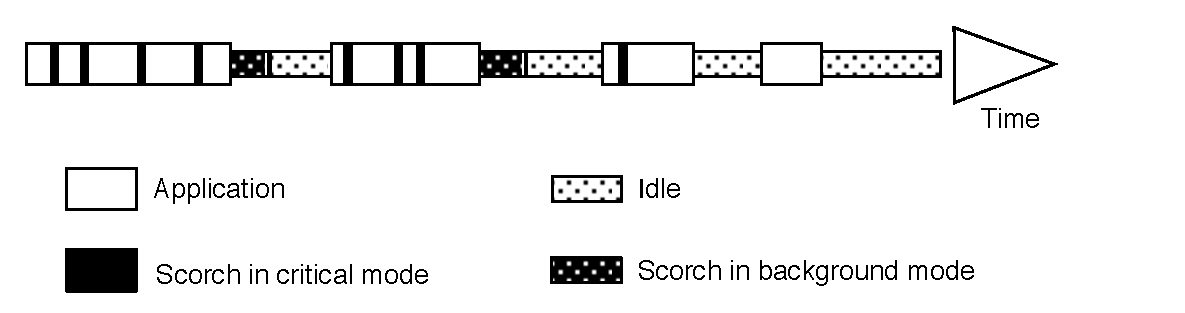
\includegraphics[width=0.9\linewidth]{ScorchModes}
        \caption{Scorch critical and background modes}
        \label{fig:ScorchModes}
    \end{center}
\end{figure}

%Fig explanation, critical vs background mode
As shown on figure \ref{fig:ScorchModes}, when the application is running, it can be interrupted for a small time window at worst. When the application normally becomes idle, the background green thread starts optimising the functions long to optimise. When no more functions are queued for optimisations, the application becomes idle. In any case, after a while, all critical portions of code have been optimised and the application is usually not interrupted any more while the background green thread has usually no more v-functions to optimise.

The Scorch optimiser can be run in two modes. On critical mode, it interrupts the application green thread and has a limited time-window to optimise a function. On background mode, it optimises code only when the application is idle but as no time limit. This design allow all the application's code to be optimised in a single-threaded environment without the system loosing too much responsiveness.

\subsection{Hot spot management}

%generic profiling counters
To introduce the optimising JIT, Cogit was extended to support a conditionnal compilation. Based on a specific bit in the v-function's header, Cogit compiles the v-function with or without profiling counters. Typically, non optimised v-functions, produced by the source code to v-function compiler, are by default compiled to n-functions with profiling counters, while optimised v-functions are compiled without profiling counters. Profiling counters are generated so that the counter is increased by one when the execution flow reaches it and to call a specific hot spot detection routine when the counter reaches a threshold.

%SHOW v-function header format ?

%Counters on branch
Based on \cite{Arn02}, we added counters by extending the way the baseline JIT generates conditional jumps to add counters just before and just after the branch. In several other VMs, the counters are added at the beginning of each function. The technique we used allowed us to reduce the counter overhead as branches are 6 times less frequent that virtual calls in the Smalltalk code we observe on production application. In addition, the counters provide information about basic block usage. Every finite loop requires a branch to stop the loop iteration and most recursive code requires a branch to stop the recursion, so the main cases for which we wanted to detect hot spots for are covered.

%hot spot detection - call-back
When a hot spot is detected, a specific Slang routine is called. The routine makes sure the n-frame with the tripping counter is reified or reify it so it can be introspected from Smalltalk. Then, the routine performs a virtual call with a selector specified in Smalltalk, the reified stack frame as the receiver and the boolean the conditionnal jump was branching on as a parameter. The execution stack has then a stack frame for the activation of the virtual call performed by the routine at the bottom, and the frame just above is the stack frame holding the n-function with the hot spot.
%Flag: FRAMEREIFICATION.

%returning from call-back
Just after the machine code calling the routine, Cogit generates a back jump to the conditional branch. This way, if the Smalltalk code resets the profiling counters and returns the boolean from the call-back, the application execution is resumed by performing one more time the branch with the same boolean.

%WARNING ! What happen when conditionalBranchTrip and reification.

%activating Scorch
As the routine performs a normal virtual call, the execution continues in Smalltalk. The default behavior in this method is to call the Scorch optimiser, passing the receiver (the reified stack frame holding the n-function with the hot spot).

\subsection{Scorch optimiser}

The Scorch optimiser is activated by the call-back and has access to a reification of the current stack, from the stack frame where the hot spot was detected. We call the \emph{tripping function} the function where the hot spot is detected, because a counter has "tripped" in this function. Scorch firstly analyse the stack and finds the best function to optimise. It then, either directly in critical mode or indirectly through background mode generates an optimised v-function and installs it for further uses.

\paragraph{Stack search.}
\label{ss:stackSearch}

%Function selection, bottom is bad
When Scorch is activated, it has access to a reification of the stack. A naive approach would be to always optimise the tripping function and not to search the stack at all. Unfortunately, it would be a terrible heuristic for Smalltalk. Indeed, an important part of the execution time is due to the extensive use of closures. More specifically, most loops in the executed code, assuming the code respects standard Smalltalk coding conventions, are using closures. To efficiently remove the closure overhead, the closure needs to be inlined up to its enclosing environment to remove both the closure creation and the closure activation. If the tripping function is either activating closures or a closure activation itself, then optimising it won't gain that much performance because the closure creation and activation time will remain.

%Function selection, bottom or home is bad
Another approach, a bit less naive, would be to optimise the tripping function if it is a method, and the enclosing environment's function if it is a closure, in an attempt to remove closure overhead. Yet, this heuristic does not solve either the most common case. To illustrate the problem, let's look at a simple example with a loop over an array.

%array loop example. descr exampleArrayLoop
In the code sample shown below, \ct{exampleArrayLoop} is a method installed in the class \ct{ApplicationClass}. Its method body consists of a loop over an array, the array being an instance variable. To loop over an array, Smalltalk provides high level construct such as \ct{do:}. In this case, \ct{do:} is very similar to \ct{foreach} in other languages and allows to iterate over the array while providing at each iteration of the loop the array's element in the variable \ct{element}. The \ct{do:} method takes a single argument, a closure, which is evaluated using \ct{value:} at each iteration of the loop.

\begin{code}
	ApplicationClass >> exampleArrayLoop
	    array do: [ :element | FileStream stdout nextPutAll: element printString ].
		
	Array >> do: aBlock
	    1 to: self size do: [:index | aBlock value: (self at: index)].
\end{code}

%descr do:
The method \ct{Array >> do:} is using a special selector, \ct{to:do:}, which is compiled by the bytecode compiler to a loop, in a similar way to \ct{for} constructs in other languages. In fact, this method is a loop from 1 to the size of the array. Index starts with the value 1 and is incremented by 1 at each iteration of the loop. At each iteration, the current value of index is tested against the size of the array, and when that value is reached the loop is exited.

%profiling counter location
As discussed in the previous section, profiling counters detect frequent portion of code on branches. Each finite loop has a branch to either keep iterating over the loop or exit the loop. In the example, it means that the method \ct{Array >> do:} has a profiling counter on the branch testing the value of the index against the size of the array. The rest of the code, in the two methods and in the closure, have no other profiling counters.

%closure issue and why to pick next function
The hot spot is going to be detected on the profiling counter, hence in the method \ct{Array>>do:}. As we said before, an important part of the execution time is spent creating and evaluating the closure. From the \ct{Array>>do:} method, it is not possible to know what closure will be executed as the closure is an argument. However,  \ct{Array>>do:} gets inlined into \ct{ApplicationClass>>exampleArrayLoop}, the closure evaluated is known to be the closure created in  \ct{ApplicationClass>>exampleArrayLoop}. Hence, to gain maximum performance, the optimiser should decide to optimise \ct{ApplicationClass>>exampleArrayLoop} and inline both the \ct{Array>>do:} method and the closure evaluation (\ct{value:}). 

%detail of the problem
We note that in this case, the tripping function would be \ct{Array>>do:}. The tripping function is therefore a method, not a closure, and yet it is better to pick the caller stack frame's function for optimisations.

%closure last explanation
Overall, because of the extensive use of closures, the optimiser almost never picks the tripping function for optimisation. It usually walks up a few frames to find the best function to optimise. 

\paragraph{Optimised v-function generation.}
Once Scorch has selected the v-function to optimise, it generates an optimised v-function. It attempts to do it immediately, within a limited amount of time. If it fails to do it, it postpones the optimisation to background mode. The function's optimisation and installation is using the same code in both cases, so we will discuss only the critical mode optimisation in the following paragraph.

Scorch's optimiser is implemented with traditional compiler optimisation techniques. It decompiles the v-function to optimise into a single static assignment intermediate representation, represented in the form of a control flow graph. Specific instructions that may require deoptimisation of the optimised stack frame have deoptimisation metadata attached which is updated across the optimisation process to still refer to the right values. The same intermediate representation is used during the whole optimisation process.

Scorch's optimiser then performs Smalltalk specific optimisations, very similar to the ones present in optimising JITs for other object languages. It starts with function inlining. For each inlined v-function, the v-function is decompiled to the same intermediate representation and merge into the same control flow graph. Once the inlining phasis is done, it performs standard optimisations such as array-bounds check elimination with the ABCD algorithm (CITE), global value numbering, loop invariant code motion.

All the optimisations are guided by previous runs of the functions: Scorch can ask Cogit for each v-function (the optimised one and the inlined ones), if it was compiled to a n-function by Cogit, to introspect the machine code and provide type information for each virtual call based on the data present in the corresponding inline cache and provide basic block usage based on the profiling counter values.

The back-end is the only non conventionnal part of the optimiser. Scorch needs to generate an optimised v-function. Most instructions maps one to one to the extended bytecode set instructions, but the back-end still needs to map the intermediate instructions to stack-based instruction by figuring out which value can simply be on stack and which value needs to be put in a temporary variable slot and update correctly the deoptimisation metadata.

At the end of the process, an optimised v-function is generated. The optimised v-function has attached deoptimisation metadata. For each point where deoptimisation could be requested (typically, failing guards, but also each virtual call for debugger support), the optimised v-function has metadata to reconstruct the stack with non optimisedv-function.

\paragraph{Installation.}
If the optimisation has been done in time in critical mode or has simply been done in background mode, the optimised v-function can be installed. It is installed in the method dictionary of a class if this is a method, or in a method if it's a closure. If an optimised method is installed, the installation explicitely requests the VM to flush the caches dependent of this installation (the global look-up cache for the interpreter and the inline caches).

In addition, the dependencies are installed in the dependency manager so that if new code is loaded, code that may be dependent is discarded.

Once installed, conceptually, the VM runs the optimised v-function as normal v-function. The first few runs is interpreted and the subsequent runs use the n-function produced by Cogit. The only difference is that optimised v-functions have access to additional operations, but those operations are supported both by the interpreter and by Cogit. The first version we had running was working exactly this way.

We then added a cheap heuristic to encourage the execution of optimised v-functions as n-functions. Optimised v-functions have a bit set in their header to tell Cogit not to compile profiling counters when generating their corresponding n-function. If this bit is set, we added the heuristic that the interpreter asks Cogit to compile it at the first run and immediately uses the n-function. 

In any case, the VM still needs to support the interpretation of optimised v-functions. Indeed, in very rare cases, Cogit cannot temporarily generate a n-function for the given v-function. For example, as the native code zone for n-functions has a fixed size of a few megabytes, it can happen that Cogit tries to compile a v-function while relinking a polymorphic inline cache (CITE) of another n-function. If there is not enough room in the machine code zone, a compaction of the machine code zone has to happen while generating the n-function. It is not easy to compact the machine code zone at this point as it can happen that the polymorphic inline cache or the n-function referring it is discarded. To keep things simple, in this situation, we postpone the the machine code zone compaction to the next interrupt point and interpret the v-function once.

%%%%%%%%%%%%%%%%%%%%%%%%%%%%%%%%%%%%%%%%%%%%%%%%%%%%%%%%%%%%%%%%%%%%%%%%%%%%%%%%%%%%%%%%%%%%%%%%%%%%%%%%%%%%%%%%%%%%%%%%

\section {Function's deoptimisation}

%intro
The deoptimisation of the execution stack is similar to other virtual machines \cite{Fin03a, Holz92a}. The optimised frame is on stack and is in most case a n-frame. It cannot be used any more because an optimisation time assumption is invalid at runtime (a deoptimisation guard has failed) or the optimised function was discarded (by the debugger or because of new code loading). Deoptimising the stack requires the mapping of the optimised frame to multiple non optimised v-frames. 

%Main difference
On the contrary to most other VMs, deoptimisation is done in two steps. Firstly, Cogit deoptimises the optimised n-frame to a single optimised v-frame. This step is not performed in the very uncommon case where deoptimisation happens already from an optimised v-frame. Secondly, Scorch deoptimises the optimised v-frames to multiple non optimised v-frames.

%only stack deopt
When discussing deoptimisation, we deal only with stack recovery (deoptimisation of the bottom optimised frame to the non optimised v-frames). The non optimised v-function is always present and never discarded, so it can be directly set in the non optimised v-frames restored during the deoptimisation process. There is no such thing in our design and implementation as reconstructing non optimised v-function from optimised v-function based on deoptimisation metadata. As far as we know, modern VMs such as V8~\cite{V8} always keep a non-optimised version of each function, so we believe the memory footprint impact of keeping them is acceptable.

\subsection{Deoptimisation management}

%Intro + 2 cases.
Deoptimisation can happen in two main cases. Firstly, Scorch's optimiser inserts guards to ensure assumption taken a optimisation time are valid at runtime, such as the speculation on types. Such guards can fail, requiring doptimisation of the execution stack to keep executing the application correctly. Secondly, Smalltalk code can require deoptimisation of the code through the use of the reified stack frames APIs. Typically, Smalltalk code requests deoptimisation for debugging but it could request it for other purpose.

\paragraph{Guard failure.} When a guard fails, the native code generated by Cogit (or the interpreter in case of a guard failure in an optimised v-frame) calls a specific routine in Slang to perform the deoptimisation of the stack. The routine makes sure the frame with the tripping counter is reified or reify it so it can be introspected from Smalltalk. Then, the routine performs a virtual call with a selector specified in Smalltalk and the reified stack frame as the receiver. The execution stack has then a stack frame for the activation of the virtual call performed by the routine at the bottom, and the frame just above is the optimised frame requesting deoptimisation. 

%low-level stack banging issue, in Slang ?
%Flag: FRAMEREIFICATION.

\paragraph{Smalltalk code deoptimisation.}The Smalltalk code can request deoptimisation of specific frames to perform specific operations such as debugging. In this case, the situation is different because the frame to deoptimise is not necessarily the bottom frame and its instruction pointer is not on a guard instruction. All instructions where deoptimisation can happen are annotated with deoptimisation metadata, so having the instruction pointer on a non guard instruction does not really change anything in the deoptimisation code. Having the stack frame in the middle of the stack is, however, quite annoying and is discussed in the next section.

%TODO REWRITE PREV  Because of deopt frames, we're never in a case where bottom frame. 

\subsection{Scorch deoptimiser}

%deopt through metadata 
Scorch's deoptimiser is activated on an optimised v-frame (an optimised n-frame would have been reified by Cogit to an optimised v-frame). It is necessarily activated on a virtual instruction which is annotated with deoptimisation metadata. The metadata consists of a list of objects to materialize, which allocation have been postponed from runtime to deoptimisation time. As v-frames are reified as objects, part of those objects to rematerialize are in fact non optimised v-frames. For each field of each object, the metadata specifies if the value is a specific constant, a value to fetch in the optimised v-frame or a reference to one of the other rematerialized object.

\paragraph{Stack edition.}

%TODO rewrite next. Because of deopt frames, we're never in a case where bottom frame. 

Once all the non optimised v-frames are reconstructed, the execution stack needs to be edited to use them. The most common case, and the most critical for performance, happens when a deoptimisation guard fails. In this case, the frame to deoptimise is the bottom frame. We can therefore simply pop it and push the deoptimised frames.

%complex stack edition
However, if deoptimisation was requested by Smalltalk code and not by a guard, the frame to deoptimise may not be the bottom stack frame. In this case, the VM needs to split the current stack page in two, copying one part on another stack page. This way, some room is freed to insert multiple frames (potentially, a third stack page could be inserted in between if many frames have to be restored). This operation was already supported and used in Smalltalk to implement continuations and exceptions without VM support, so we simply re-used the feature.

\paragraph{Discard functions.} When new functions are installed (for example when a library is loaded), optimisation assumptions may be invalidated because some look-up result cannot be guaranteed any more. In this case, we cannot really iterate over the whole stack nd deoptimise all the frames holding invalidated code as it would take a long time. Instead, Scorch mutates the optimised v-function to discard so they hold only guard failures instructions and requests Cogit to patch all return instruction pointers of all optimised n-frames with a discarded function to an instruction pointer in a speific routine which will trigger deoptimisation upon return.

\paragraph{Execution restart.}

If the deoptimisation happened due to a guard failure (or due to a return to a discarded function), the application needs to resume execution once deoptimisation is performed. In those cases, the first deoptimiser frame is just below the bottom restored non optimised v-frame. Returning from the deoptimiser frame to the application is not as easy as for the optimiser call-back. The optimiser is always triggered on a conditional branch and conditionnal branches require a value to test to be on stack. Hence, the optimiser could simply return the value to test and the execution resumes just before the branch. 

In the case of deoptimisation, the application stack frame could be restored on many different instructions. Especially, it could be restored at an instruction where no value is on stack. Hence to return to the application, the deoptimiser has to perform a special return instruction, which resumes the caller frame execution without pushing any value on its frame.

%%%%%%%%%%%%%%%%%%%%%%%%%%%%%%%%%%%%%%%%%%%%%%%%%%%%%%%%%%%%%%%%%%%%%%%%%%%%%%%%%%%%%%%%%%%%%%%%%%%%%%%%%%%%%%%%%%%%%%%%

% \section {Conclusion} ?


\ifx\wholebook\relax\else
    \end{document}
\fi